\begin{question}
Given the historical series of three stock prices in the file
$\href{https://raw.githubusercontent.com/matteosan1/finance_course/develop/libro/input_files/historical.csv}{\textrm{historical.csv}}$
compute the 1-day 95\% VaR for a portfolio consisting of 40 FOX shares, 35 ABC shares and 25 CBS shares. 
Today's price is the last entry of the series.

\noindent\textbf{Hint:} when simulating the historical scenarios take care of possible NaN values
in the series. 
\end{question}

\cprotEnv\begin{solution}
\begin{ipython}
import pandas as pd
import numpy as np

df = pd.read_csv("https://raw.githubusercontent.com/matteosan1/finance_course/develop/libro/input_files/historical.csv")
df['FOX_RETS'] = np.log1p(df['FOX'].pct_change())
df['CBS_RETS'] = np.log1p(df['CBS'].pct_change())
df['ABC_RETS'] = np.log1p(df['ABC'].pct_change())
\end{ipython}
\begin{ioutput}
         date    FOX    CBS    ABC  FOX_RETS  CBS_RETS  ABC_RETS
0  2018-03-27  36.08  52.35  84.01       NaN       NaN       NaN
1  2018-03-26  36.58  51.69  84.95  0.013763 -0.012688  0.011127
2  2018-03-23  35.45  49.27  84.03 -0.031378 -0.047949 -0.010889
3  2018-03-22  36.18  50.26  85.00  0.020383  0.019894  0.011477
4  2018-03-21  36.30  50.87  89.50  0.003311  0.012064  0.051587
\end{ioutput}
\begin{ipython}
w = np.array([0.4, 0.35, 0.25])

df = df.dropna()
dP = []
current_value = df[['FOX', 'ABC', 'CBS']].iloc[-1].values
for i in range(len(df)):
    variation = (current_value * df[['FOX_RETS', 'ABC_RETS', 'CBS_RETS']].iloc[i])
    dP.append(variation.dot(w))

hist_var = np.percentile(dP, 1)
print ('Historical VaR is  {:.3f}'.format(hist_var))\end{ipython}
\begin{ioutput}
Historical VAR is -1.385
\end{ioutput}
\begin{figure}[htbp]
	\centering
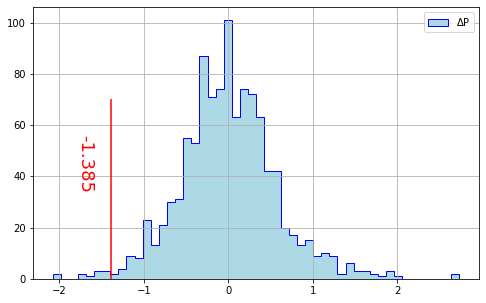
\includegraphics[width=0.7\linewidth]{figures/hist_var_ex}
\end{figure}
\end{solution}

\begin{question}
You have a 3-years call with strike \euro{110}. The underlying initial price is \euro{100} and the mean rate of return is 0.05 with a volatility of 0.15. The risk-free rate is 0.03 flat.
Compute the CVA of the contract assuming a recovery rate of 40\% and default probabilities for the underlying of 10\%, 20\% and 30\% for first, second and third year respectively.
\end{question}

\cprotEnv\begin{solution}
Below ten simulations of the underlying price in the next three years.

\begin{figure}[htbp]
	\centering
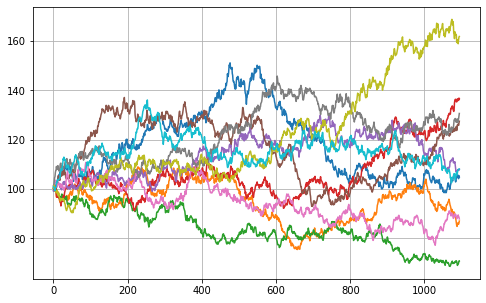
\includegraphics[width=0.7\linewidth]{figures/underlying_simulation}
\end{figure}
This is a first implementation of the CVA calculation, not optimized in terms of speed. It takes about 700 seconds to run 1000 simulations.

\begin{ipython}
from datetime import date
from dateutil.relativedelta import relativedelta
from finmarkets import call_price, CreditCurve
from scipy.stats import norm
import numpy as np
import time

np.random.seed(1)
dt = 1/365
K = 110
sigma = 0.15
mu = 0.05
r = 0.03
T = 3
R = 0.4
S = [1, 0.9, 0.8, 0.7]
obs_date = date.today()
pillars = [obs_date + relativedelta(years=i) for i in range(T+1)]
cc = CreditCurve(pillars, S)
t1 = time.time()
scenarios = 1000
cvas = []
St = S0*np.ones(shape=(T*365, scenarios))
for s in range(scenarios):
    cva = 0
    St = 100
    for t in range(0, 365*T):
        St = St * np.exp((mu - 0.5 * sigma**2) * dt + sigma
            * np.sqrt(dt) * norm.rvs(size=1))
        cva += call_price(dt*t, St, K, r, sigma, T)
            *(cc.ndp(obs_date+relativedelta(days=t))-
            cc.ndp(obs_date+relativedelta(days=t+1)))

        cvas.append(cva*(1-R))

print (np.mean(cvas))
print (time.time()-t1)
\end{ipython}
\begin{ioutput}
\end{ioutput}
The next implementation, the one actually used, exploits the \texttt{numpy.array} and it is about 30\% faster.

\begin{ipython}
from datetime import date
from dateutil.relativedelta import relativedelta
from finmarkets import call_price, CreditCurve
from scipy.stats import norm
import numpy as np
import time

np.random.seed(1)
dt = 1/365
K = 110
sigma = 0.15
mu = 0.05
r = 0.03
T = 3
R = 0.4
S = [1, 0.9, 0.8, 0.7]
obs_date = date.today()
pillars = [obs_date + relativedelta(years=i) for i in range(T+1)]
cc = CreditCurve(pillars, S)
t1 = time.time()
scenarios = 1000
cvas = []
St = S0*np.ones(shape=(T*365, scenarios))
for i in range(T*365):
    norms = norm.rvs(size=scenarios)
    St[i, :] = St[i-1, :] * np.exp((mu - 0.5 * sigma**2) * dt + sigma
        * np.sqrt(dt) * norms[:])

for s in range(scenarios):
    cva = 0
    for t in range(365*T):
        cva += call_price(dt*t, St[i, s], K, r, sigma, T)* \
            (cc.ndp(obs_date+relativedelta(days=t))-
             cc.ndp(obs_date+relativedelta(days=t+1)))

        cvas.append(cva*(1-R))

print (np.mean(cvas))
print (time.time()-t1)
\end{ipython}
\begin{ioutput}
3.7521017896018973
459.46695613861084
\end{ioutput}
\end{solution}

\begin{question}
Consider a 1-years call with strike \euro{110}. The underlying initial price is \euro{100} and the mean rate of return is 0.05 with a volatility of 0.15. The risk-free rate is 0.03 flat.
Compute the 99.9\% Credit VaR assuming a recovery rate of 40\% and default probabilities for the underlying of 30\% within next year.
\end{question}

\cprotEnv\begin{solution}

\begin{ipython}
# 460s for 1000 simulations
from datetime import date
from dateutil.relativedelta import relativedelta
from finmarkets import call_price, CreditCurve
from scipy.stats import norm
import numpy as np

np.random.seed(1)
dt = 1/365
K = 110
sigma = 0.15
mu = 0.05
r = 0.03
T = 1
R = 0.4
S = [1, 0.7]
obs_date = date.today()
pillars = [obs_date + relativedelta(years=i) for i in range(T+1)]
cc = CreditCurve(pillars, S)
scenarios = 1000
losses = []
St = S0*np.ones(shape=(T*365, scenarios))
for i in range(T*365):
    norms = norm.rvs(size=scenarios)
    St[i, :] = St[i-1, :] * np.exp((mu - 0.5 * sigma**2) * dt + sigma
        * np.sqrt(dt) * norms[:])

for s in range(scenarios):
    loss = 0
    for t in range(365*T):
        loss += call_price(dt*t, St[i, s], K, r, sigma, T)* \
            (cc.ndp(obs_date+relativedelta(days=t))-
             cc.ndp(obs_date+relativedelta(days=t+1)))

        losses.append(cva*(1-R))

print (np.percentile(cvas, [99.9]))
\end{ipython}
\begin{ioutput}
[9.96586061]
\end{ioutput}

\begin{figure}[htbp]
	\centering
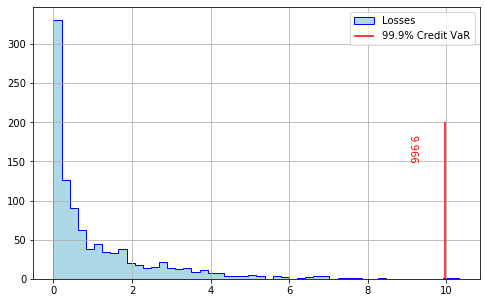
\includegraphics[width=0.7\linewidth]{figures/cr_var_ex}
\end{figure}
\end{solution}





